\subsection{Excercise MicroArchDMCar}
This task introduces the microarchitecture of the DM-CarV1.0 microservice.
First, the general structure of a microarchitecture is explained.
Then, the structure of the DM-CarV1.0 microarchitecture is shown and explained.
Finally, the microarchitecture is visualized in VS Code.

\subsubsection*{Parts of a Micro Architecture}
The microarchitecture specifies the internal code structure of the microservice.
It plays a major role in the further development and maintenance process whether on the chosen complexity.
The basic structure of a microservice's microarchitecture is divided into three separate parts: the Microservice Requester, the Microservice API, and the Persistency Interface.
Each of these parts is described in more detail in the following.

\paragraph*{Microservice Requester:}
The Microservice Requester is the software unit sending requests to the microservice and receiving the microservice's responses.
This can be the front end or another microservice.

\paragraph*{Microservice API:}
Each microservice implements and provides an API.
It is defined by the microservice's specification and is usually based on REST or gRPC depending on the microservice's requirements.
The API contains the Domain or Application logic, based on the type of microservice.
It implements the according operations and logic.
The logic is structured according to the given operations.

\paragraph*{Persistency Interface:}
This part provides the data elements like entities or value objects.
These elements can be accessed by the operations.
This enables decoupling of the interface to the database by which the data elements are stored.

\subsubsection*{Parts of the DM-CarV1.0 Micro Architecture}
The general structure of a microarchitecture has been explained in the previous section.
This task applies the general structure to the DM-CarV1.0 microservice.
The structure of the DM-CarV1.0 microarchitecture is shown in \autoref{fig:ms_dmCar_microArchitecture}.

\paragraph*{Microservice Requester:}
The DM-CarV1.0 microservice does not have a requester in this implementation.
Yet, another microservice or the front end could be the requester if the microservice is used in a real-world scenario or the microservice is extended.
Therefore the requester is not included in the graphics.

\paragraph*{Microservice API:}
The microservice API consists of the controller and the specification.
The specification is the OpenAPI specification of the microservice and describes the endpoints and operations of the microservice.
The controller implements the paths of the specification by calling the operations from the operations package.

\paragraph*{Models and Operations:}
This layer implements the domain logic of the microservice.
It contains the operations and the models.
The model package contains the entities and value objects as specified in the API diagram.
The operations package contains the operations and their according tests.
Each operation is implemented in a separate file to ensure the separation of concerns.

\paragraph*{Persistency Interface:}
The persistency interface is implemented in the \texttt{infrastructure} package.
It contains the mappers, the persistence entities, and the repositories.
The mappers provide the functions to convert \texttt{car} and \texttt{cars} model objects to persistence entities and vice versa.
The persistence entities are the entities that are stored in the database.
The repositories provide the functions to interact with the database and the in-memory repository.

\begin{figure}
    \centering
    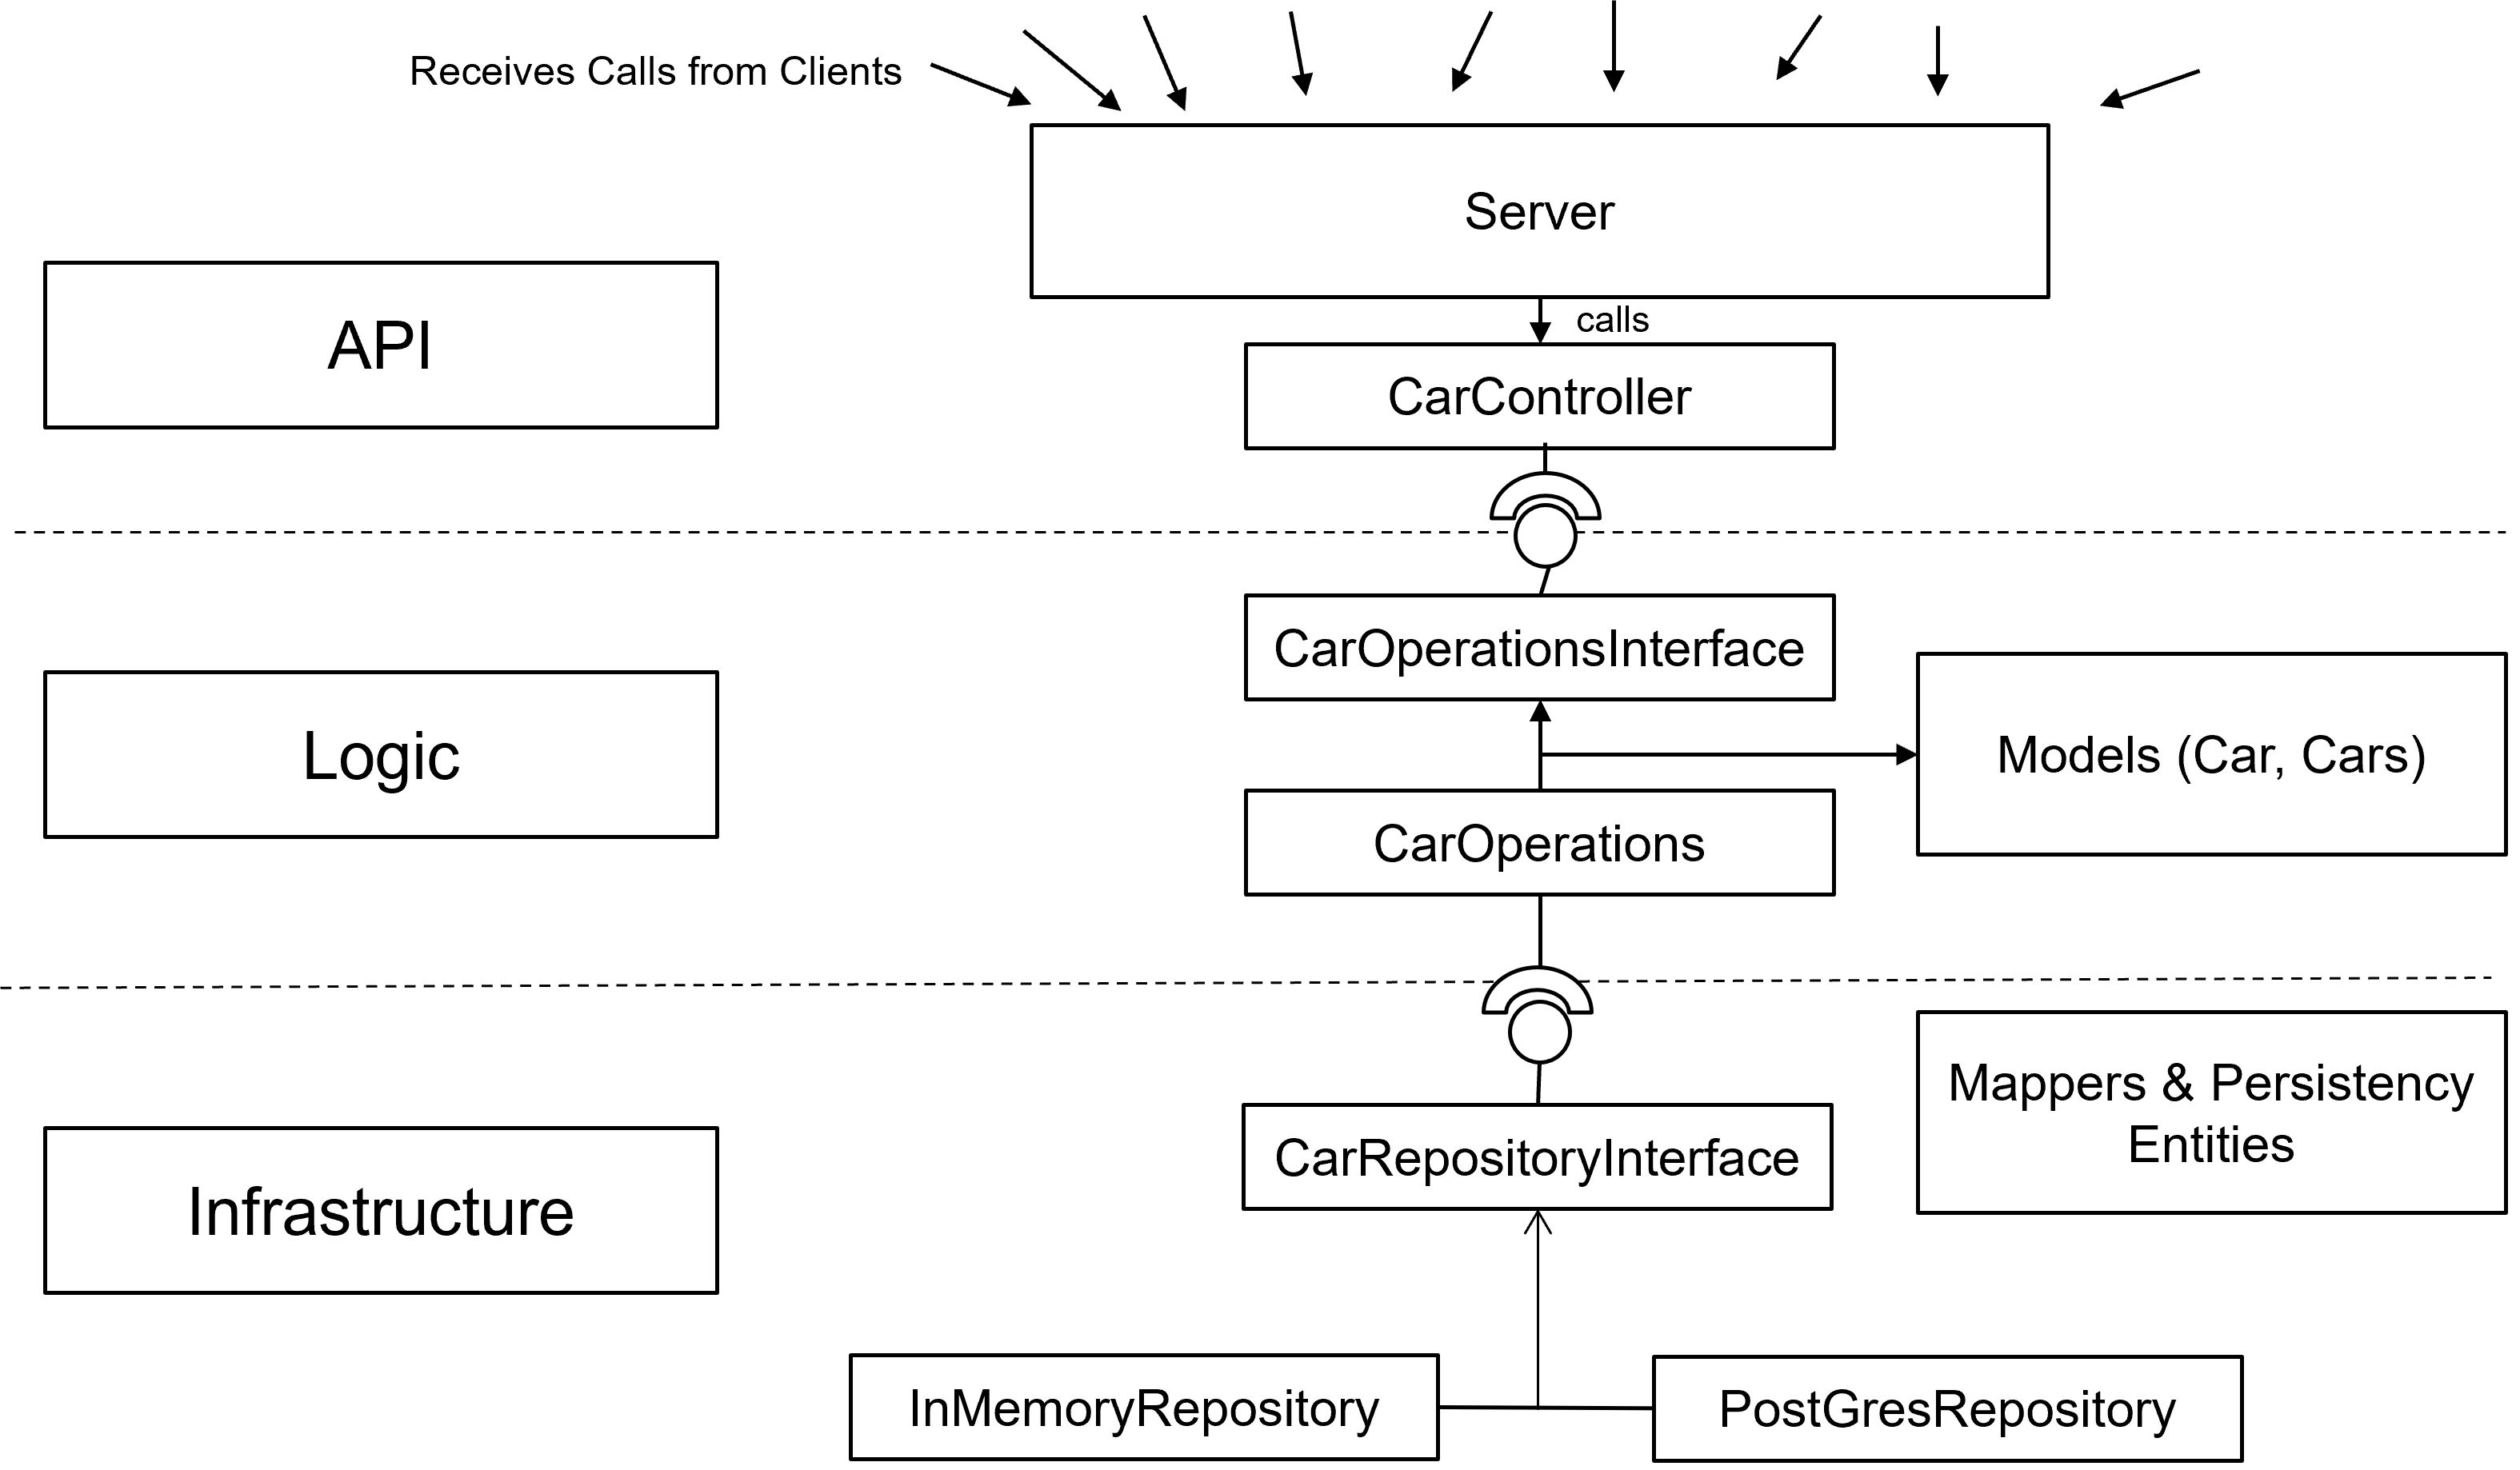
\includegraphics[width=0.8\textwidth]{figures/microservices/dmCar/ms_dmCar_microArchitecture.png}
    \caption{Micro Architecture of the DM-CarV1.0 Microservice}
    \label{fig:ms_dmCar_microArchitecture}
\end{figure}

\subsubsection*{Micro Architecture in VS Code}
//TODO: ???

%====================================================

\subsection{Excercise LogicPartDMCar}
This task dives deeper into the microarchitecture of the DM-CarV1.0 microservice.
Parts of the microarchitecture are explained in greater detail.

\subsubsection*{Content of the Logic Folder}
% Primary aspects of the logic folder
As previously explained, the logic folder contains the domain logic of the microservice.
It implements the API diagram that was shown in the previous tasks.
% Purpose of different subfolders and their go files?
The logic folder is separated into two subfolders: the model and the operations.
The model folder contains the entities and value objects.
It also contains the \texttt{CarRepositoryInterface} that is implemented in the operations folder.
Also, the test data, a collection of data for testing, is stored in the model folder.
Every other file in the model folder contains one entity or value object.

The operations folder contains the operations and their tests.
Each operation is implemented in a separate file to ensure the separation of concerns.
Also, each test is implemented in a separate file.

Therefore, the subfolders' task is to separate the entities and value objects from the operations and their tests.
This ensures the separation of concerns and the single responsibility principle.
Also, the separation becomes clearer and the code is easier to maintain.

\subsubsection*{Repository Interface}
% Description of the CarRepositoryInterface
The \texttt{CarRepositoryInterface} is placed in the \texttt{logic/model} folder.
It provides the signatures of the functions \texttt{GetCars} and \texttt{GetCar}.
\texttt{AddCar} will be implemented later.

% Which operations must be provided by a repository implementation
The \texttt{CarRepositoryInterface} is used to create the \texttt{CarOperations} object, which will later be used to implement the \texttt{CarController} object.
The \texttt{CarController} will be explained in more detail in the next task.
% Why is the interface located in the logic folder
Each function of the \texttt{CarRepositoryInterface} is implemented in the \texttt{operations} package with each function having a separate file.
This is done by using the \texttt{CarOperations} struct, which calls the functions from the \texttt{operations} package.
Therefore the \texttt{CarRepositoryInterface} is used to define the functions that are implemented in the \texttt{operations} package and can be called using the \texttt{CarController} struct.
Thus, it is a good choice to place the \texttt{CarRepositoryInterface} in the \texttt{logic} folder to ensure the logic is separated from the different packages.

\subsubsection*{Operations Interface}
\label{sec:operationsInterface}
% Description of the Operations Interface + which operations are provided
The \texttt{CarOperationsInterface} is placed in the \texttt{logic/model} folder.
It provides the signatures of the functions \texttt{GetCars} and \texttt{GetCar}.
\texttt{AddCar} will be implemented later.

The difference between the \texttt{CarRepositoryInterface} and the \texttt{CarOperationsInterface} is the signatures they use:
While \texttt{GetCars} has the same signature and return type, \texttt{GetCar} takes a string representing the \texttt{vin} as input, while the \texttt{CarRepositoryInterface} takes the actual \texttt{vin} value object as input.

% Which struct implements it
This interface is implemented in the \texttt{controller} package by the \texttt{CarController} struct.
This happens in the \texttt{CarController.go} file.
To create a new \texttt{CarController} object, the \texttt{CarOperations} object is needed.
The \texttt{CarOperations} object was explained in the previous task.
In \texttt{CarController.go} all the functions of the \texttt{CarOperationsInterface} are implemented.
They are implemented by calling the functions of the \texttt{CarOperations} object.
Each function represents a path of the API specification, like \texttt{/cars} or \texttt{/cars/\{vin\}}.

Wrapping things up, the \texttt{CarOperationsInterface} is used to define the layout of functions representing the API's path implementation.

\subsubsection*{Operation GetCar}
% Description of the GetCar Structure
The \texttt{GetCar} operation is implemented in \texttt{GetCarOperation.go}, which is located in the \texttt{operations} package.
It imports the \texttt{logic/model} and the \texttt{errors} package.
It then defines the \texttt{GetCar} function, which takes a string representing the \texttt{vin} as input and returns a \texttt{Car} object and an error.

First, the \texttt{vin} is converted to a \texttt{vin} value object.
Then, it is checked whether the \texttt{vin} is valid.
If it is not valid, an error is returned.
If it is valid, the \texttt{vin} value object is used to retrieve the \texttt{Car} object from the repository.
If this fails, an error is returned, otherwise the \texttt{Car} object and \texttt{nil} for the error is returned.

% Why is it possible to implement the operation in a separate file
The implementation of the operations via the \texttt{CarOperations} struct allows the implementation in a different file.
The \texttt{GetCar} function can be called via the \texttt{CarOperations} struct using the dot notation.
Therefore, the \texttt{GetCar} function can be called via \hfill \linebreak \texttt{CarOperations.GetCar(vin string)}.
\texttt{CarOperations} implements the \hfill \linebreak \texttt{CarOperationsInterface} and therefore the \texttt{GetCar} function.
By creating a \texttt{CarOperations} object, as it is done in the main function, the \texttt{GetCar} function can be called.
Therefore, it is possible to implement the operation in a separate file.

% Is it reasonable to provide every operation in a separate file
It is reasonable to provide every operation in a separate file due to the SoC principles.
Separation of Concerns (SoC) stipulates that a microservice should be broken down into smaller, individual components, each handling a single task only.
By separating the operations into different files, the SoC principles are followed.
%====================================================
\subsection{Excercise APIPartDMCar}
This task takes a close look into the \texttt{api} package of the DM-CarV1.0 microservice.
First, the content of the API folder is explained.
Then, the generated files are explained.
Afterwards, the \texttt{CarController.go} file and its differences from the generated files are explained.
Finally, the \texttt{GetCar} method of the \texttt{CarController} is explained.
Also, the Echo framework is quickly introduced, further details can be found in \autoref*{sec:the_echo_framework}.
\subsubsection*{Content of the API Folder}
% Describe primary aspects of the API folder
The API folder contains two subfolders: \texttt{controller} and \texttt{specification}. \linebreak
The \texttt{specification} folder contains the OpenAPI specification of the microservice stored in a YAML file.
\texttt{controller} contains the \texttt{CarController} struct in the \texttt{CarController.go} file and the according test file.
Furthermore, it contains primitives to interact with the OpenAPI HTTP API.
Also, a \texttt{MockEchoContext} is provided to mock a running HTTP server for testing purposes.
It can be used to test the API without starting the microservice.

% What is the purpose of the different folders
As mentioned previously, the \texttt{api} folder is separated into \texttt{controller} and \texttt{specification}.
This separation provides a clear structure, providing modularity and separation of concerns due to every package having a clear set of tasks.
This provides better maintainability, readability and testability.
Also, the documentation is improved due to the separation of concerns.
Therefore it is a good choice to separate the \texttt{api} folder into these two subfolders.
\subsubsection*{Generated Files}
% Description of the content of the generated files
The \texttt{controller} package contains two generated files: \texttt{server.gen.go} and \hfill \linebreak \texttt{server-model.gen.go}.
Both files contain the primitives to interact with the HTTP API based on the OpenAPI specification.
An HTTP API is an API that is accessed via HTTP requests, in this case, \texttt{GET} and \texttt{POST} requests.
However, the functionalities of the \texttt{POST} request will be implemented later. 

% Which framework is used
This API uses the Echo framework, which is a web framework for Go.
More on the Echo Framework can be found in \autoref*{sec:the_echo_framework}.

\paragraph*{server.gen.go}
This file delivers the functions to add each server route to register the handlers.
In this case the \texttt{GET} requests for \texttt{/cars} and \texttt{/cars/\{vin\}}.
The \texttt{main.go} file calls the \texttt{Registerhandler} function with a new echo instance and the set of functions.
These functions are then called when a request is received.
Wrapping things up, the \texttt{server.gen.go} file provides the functions to register the handlers for the incoming requests, thus creating the endpoint of the HTTP API.

\paragraph*{server-model.gen.go}
This file contains the specification of how the data is sent and received.
In this case, the \texttt{Car} struct is defined.
It is used to send the \texttt{Car} object as a response after an incoming request.
Data is sent using JSON format.
The struct defines the JSON format of the data and its properties.
Also, the identifier, here it is the \texttt{vin}, is defined.

% How do those files relate to the API specification
These files are generated based on the OpenAPI specification.
They define the routes and endpoints of the specification, as well as the data that is sent and received.
\texttt{server.gen.go} is based on the \texttt{paths} of the specification, while \texttt{server-model.gen.go} is based on the \texttt{components} of the specification.
They, therefore, represent the specification, thus they are closely related to it.

\subsubsection*{File CarController.go}
% Which interface is implemented by the CarController
The \texttt{CarController.go} file implements the \texttt{CarOpertionsInterface}.
The purpose of this interface was explained in detail in the previous tasks.

% Differences between the generated files and the CarController.go file
Taking a closer look at the \texttt{main.go} file, the differences become clear.
First, a new car controller is created by calling the \texttt{NewCarController} function.
This car controller is then passed to the \texttt{RegisterHandlers} function of the generated \texttt{server.gen.go} file.
This function registers the handlers for the incoming requests.
Therefore these files work together instead of against each other:
The \texttt{server.gen.go} file defines which functions of the \texttt{CarController} struct are called when a request is received.
\texttt{CarController} then passes the requests to the \texttt{logic} package, where the actual implementation of the operations is located.
Therefore the main difference between the generated files and the \texttt{CarController.go} file is that the generated files define the endpoints of the HTTP API, while the \texttt{CarController} defines the endpoints of the \texttt{logic} layer.

\subsubsection*{CarController's GetCar Method}
% Description of the method's signature in CarController
The \texttt{GetCar} method is implemented in the \texttt{CarController.go} file.
Its signature is listed in \autoref*{lst:getCarMethodCarController}.

First, the function is called from an existing \texttt{CarController} struct using the dot notation.
The function takes an \texttt{echo.Context} and a \texttt{vin} as input and returns an error.
The \texttt{vin} is the identifier of the \texttt{Car} object, that will be used in the further implementation of the function.
\texttt{echo.Context} is a part of the Echo framework.
It is an object representing the context of the HTTP request.
It can contain different kinds of information or data, closely correlated to the HTTP request.
This can be request information like URL or query parameters, status codes like \texttt{http.StatusOk} and much more.
Therefore it is an essential part of the function's signature.
The given context called \texttt{ctx} in the signature will also be used as a return value if the function executes correctly.
If an error occurs during execution, the error from the called \texttt{GetCar} function is returned.

\begin{lstlisting}[
    style=kit-cm,
    float=h,
    caption={Signature of the GetCar Method in CarController.go},
    label={lst:getCarMethodCarController}
]
// Route: GET /cars/:vin
func (resource CarController) GetCar(ctx echo.Context, vin Vin) error {
// Implementation
}
\end{lstlisting}
%====================================================
\subsection{Excercise InfrastructurePartDMCar}
//TODO add introduction
\subsubsection*{Content of the Infrastructure Folder}
% Describe primary aspects of the infrastructure folder
The \texttt{infrastructure} folder contains two files and two additional subfolders: \texttt{mappers} and \texttt{persistenceentities}.
A screen dump of the folder's structure is shown in \autoref*{fig:ms_dmCar_infrastructureFolder}.

% What is the purpose of the different subfolders
Each subfolder has its purpose which will be discussed in the following.
\paragraph*{mappers:}
This folder contains the \texttt{CarMapper.go} file and its test file.
It provides the functions to convert \texttt{car} and \texttt{cars} model objects to persistence entities and vice versa.

\paragraph*{persistenceentities:}
This folder contains the \texttt{CarPersistenceEntity.go} and the \texttt{EntitiesTestdata.go} files.
\texttt{CarPersistenceEntity.go} defines the car model for persistence and \texttt{EntitiesTestdata.go} provides data for testing.
\begin{figure}
    \centering
    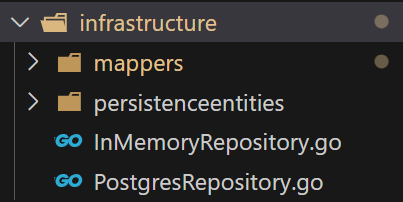
\includegraphics[width=0.5\textwidth]{figures/microservices/dmCar/ms_dmCar_infrastructureFolder.png}
    \caption{Content of the Infrastructure Folder}
    \label{fig:ms_dmCar_infrastructureFolder}
\end{figure}

\subsubsection*{Persistence Entities}
% Which persistence entities exist for DM-Car
The \texttt{car} model exists for persistence entities.
It is defined in the \texttt{CarPersistenceEntity.go} file.
All other entities are based on the \texttt{car} model, thus rendering the necessity to model further persistence entities obsolete.

% How do the persistency entries differ from the model entities
The persistence entity contains the same properties as the \texttt{car} model from the \texttt{model} folder, yet there are some differences:
Both entries differ in their usage and their purpose.
The \texttt{car} model is used to represent the data in the API, while the persistence entity is used to represent the data in the database.
The persistence entity uses more general data types like \texttt{string} or \texttt{int} instead of value objects to make it easier to store the data in the database.
That is why the \texttt{car} model contains the \texttt{vin} value object, while the persistence entity contains the \texttt{vin} as a string.
Furthermore, the persistence entity contains a structure definition using object-relational mapping.
By using the \texttt{gorm:"primaryKey"} tag, the \texttt{vin} is defined as the primary key of the database.
There is no need to use this in the \texttt{car} model since the \texttt{vin} is already defined as the identifier of the \texttt{car} model by the function usage.

Therefore, the \texttt{car} persistence entity has a specific structure for database representation.
This enables a separation between the entities of the database and the API.

\subsubsection*{Mappers}
% Description of the mappers for the CarPersistenceEntity
% What is the purpose of this mapper
As mentioned previously, a mapper is used to convert \texttt{car} and \texttt{cars} model objects to persistence entities and vice versa.
In this case, a \texttt{cars} persistence entry, just like the model entry, is a collection of \texttt{car} entities.

% Why are they required
The mappers play a crucial role in the microservice.
It allows the separation of the database from the API, therefore without the mappers the planned microarchitecture would not be possible.
This enables abstraction and decoupling.
Furthermore, mappers improve maintainability and flexibility by keeping data transformation localized.
Also, testing becomes a lot easier due to the isolation of the data transformation logic.

Therefore it is a good choice to use mappers in this microservice.

\subsubsection*{InMemoryRepository}
% Which interface is implemented by InMemoryRepository

% Where is the repository initialized and used

%====================================================
\subsection{Excercise CSGetCar}
\subsubsection*{Code Sketch GetCar}
\subsubsection*{GetCar Flow Through the Code Sketch}

%====================================================
\subsection{Challenge Operation AddCar}
\subsubsection*{Update API Diagram}
\subsubsection*{Update API Specification}
\subsubsection*{Implement Operation AddCar}
\subsubsection*{Regenerate API Server}
\subsubsection*{Implement Route at API Controller}
\subsubsection*{Complete Repository Implementation}
\subsubsection*{Run Microservice}